\section{Results}\label{sec:results}
\subsection{Voltage controlled voltage source (VCVS)}\label{sec:vcvs}

\begin{figure}[tbph]
	\centering
	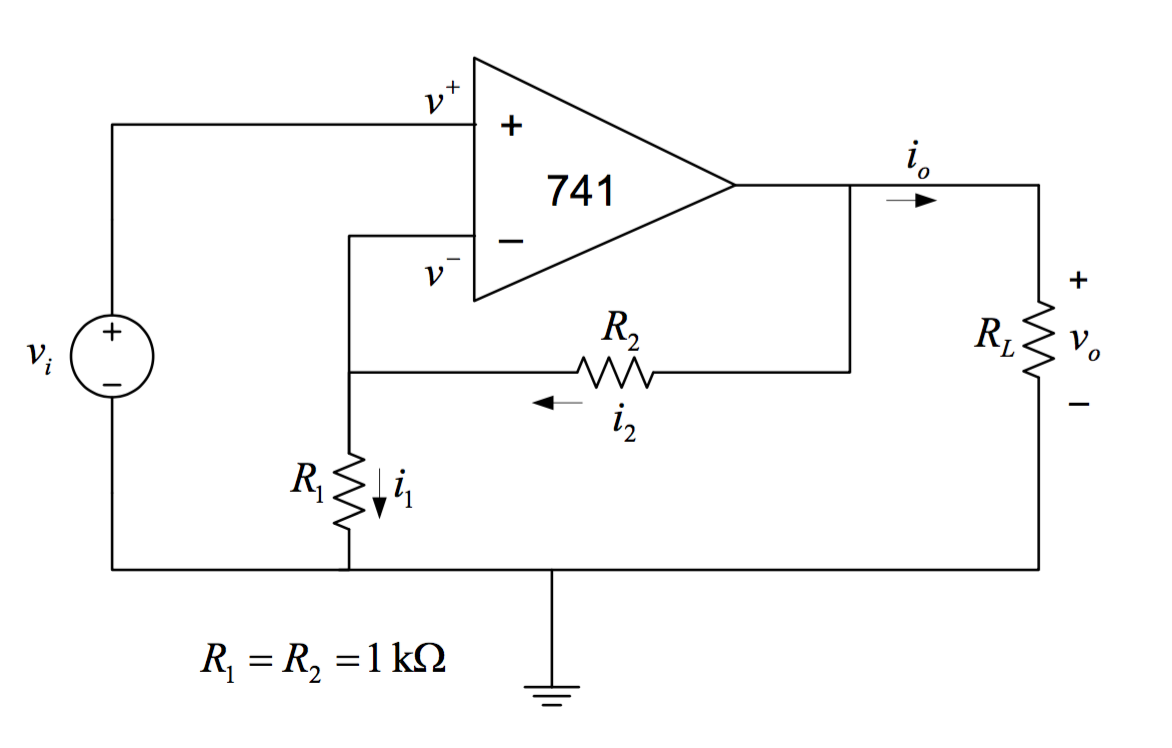
\includegraphics[width=0.7\linewidth]{graphics/vcvs-schematic}
	\caption{Schematic for VCVS with $G = 2$}
	\label{fig:vcvs-schematic}
\end{figure}

\begin{table}[htpb]
	\centering
	\begin{tabular}{@{}SS@{}}
		\toprule
		\textcol{$V_i$ (V)} & \textcol{$V_o$ (V)} \\ \midrule
		-6 & -8.467 \\
		-5 & -8.468 \\
		-4 & -8.007 \\
		-3 & -6.005 \\
		-2 & -4.003 \\
		-1 & -2.001 \\
		0 & 0.001 \\
		1 & 2.036 \\
		2 & 4.007 \\
		3 & 6.010 \\
		4 & 8.011 \\
		5 & 9.060 \\
		6 & 9.060 \\ \bottomrule
	\end{tabular}
	\caption{Response of VCVS}
	\label{table:vcvs}
\end{table}

\begin{figure}[tbph]
	\centering
	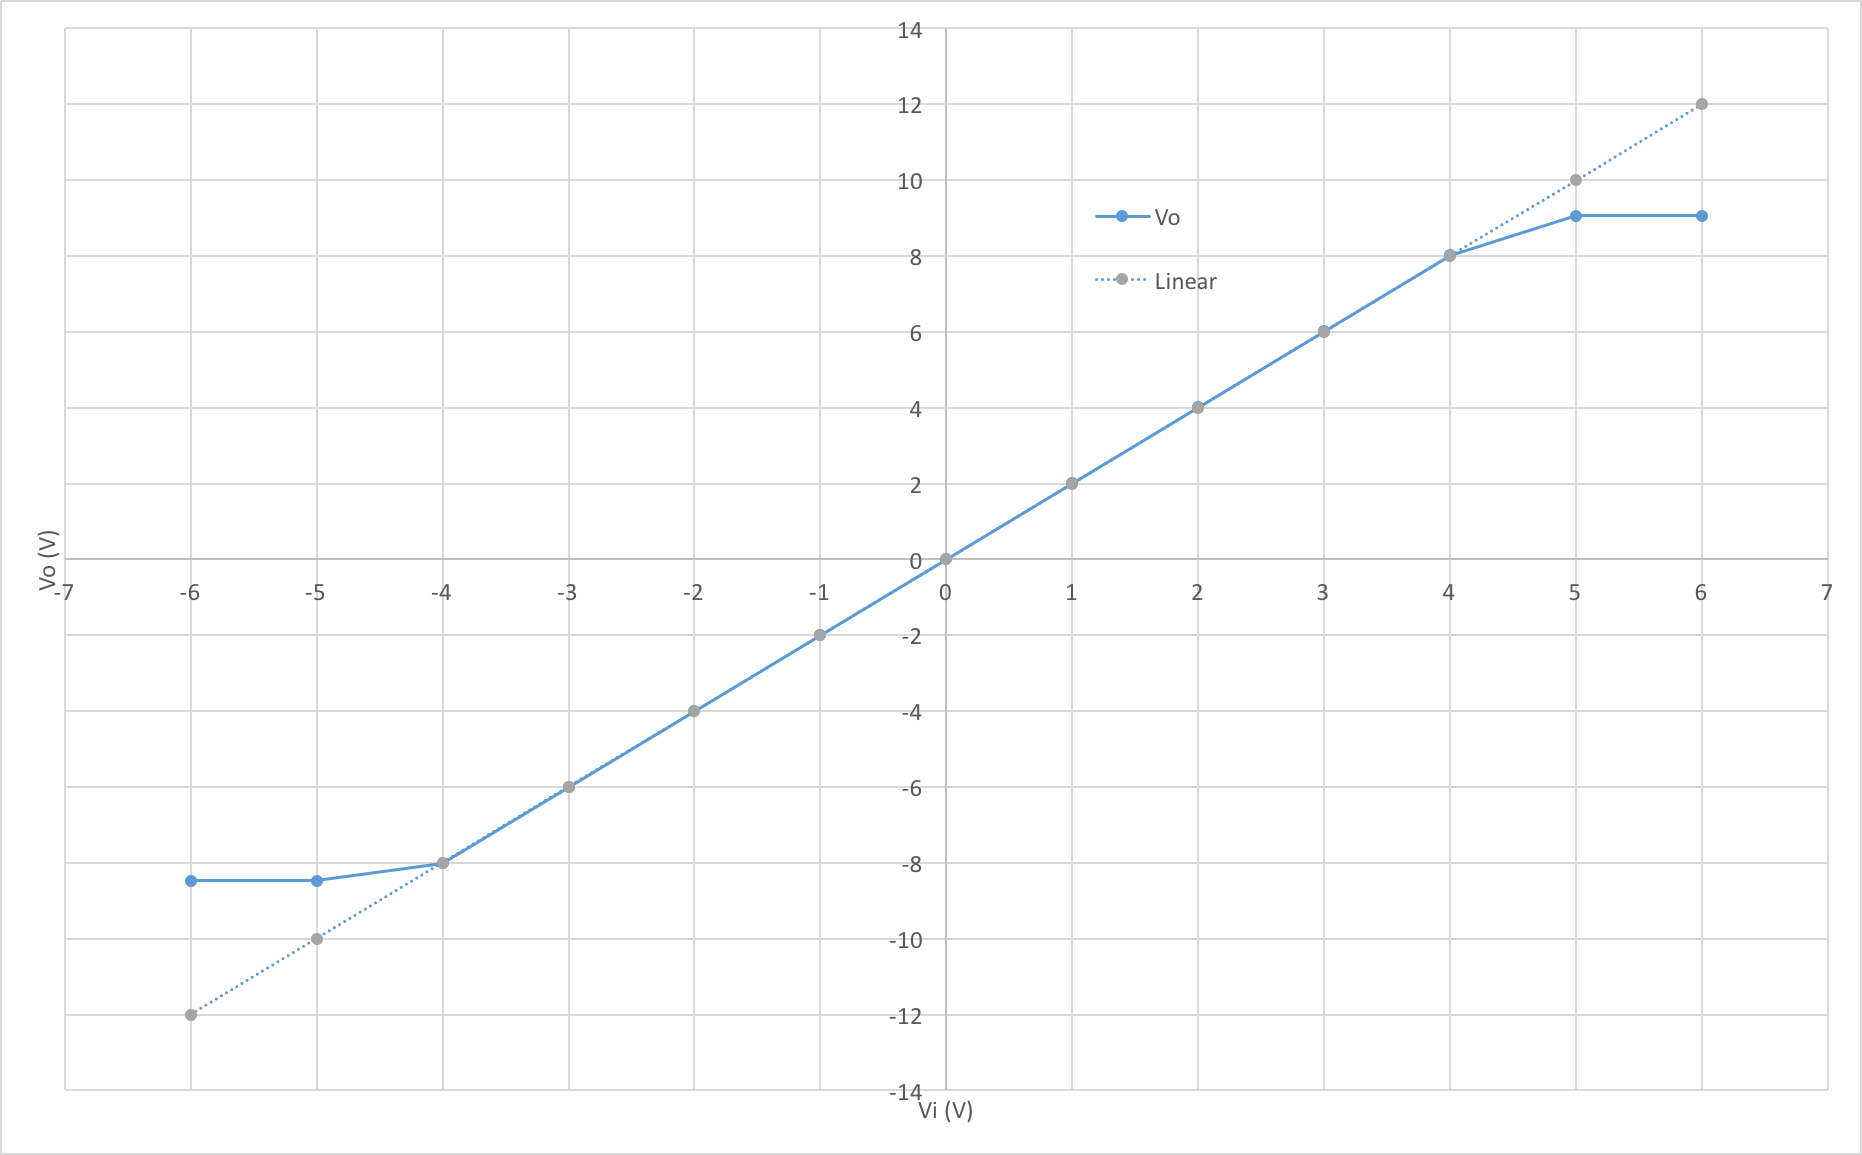
\includegraphics[width=0.95\linewidth]{graphics/vcvs-graph}
	\caption{Response characteristic of VCVS with expected linear behavior}
	\label{fig:vcvs-graph}
\end{figure}

\subsection{Voltage controlled current source (VCCS)}\label{sec:vccs}

\begin{figure}[tbph]
	\centering
	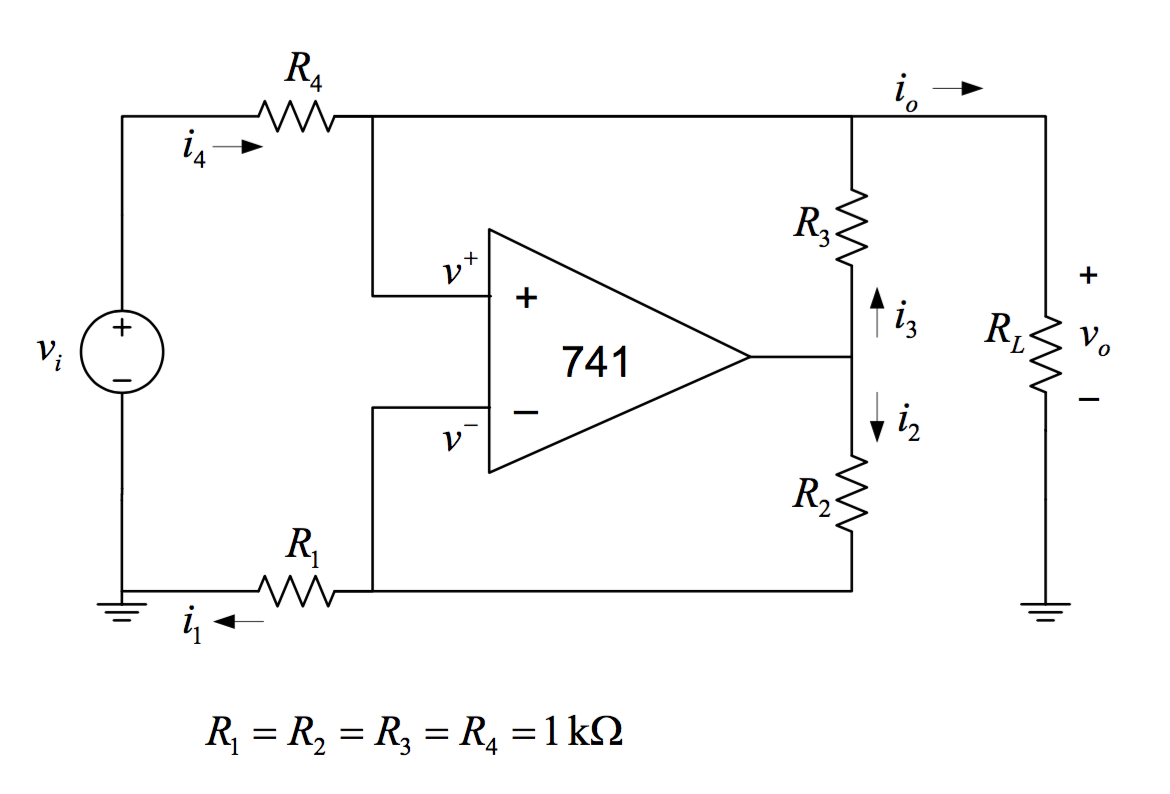
\includegraphics[width=0.7\linewidth]{graphics/vccs-schematic}
	\caption{Schematic for VCCS with $G = 1$}
	\label{fig:vccs-schematic}
\end{figure}

\begin{table}[htpb]
	\centering
	\begin{tabular}{@{}SS@{}}
		\toprule
		\textcol{$V_i$ (V)} & \textcol{$I_o$ (mA)} \\ \midrule
		-8 & -5.405 \\
		-7 & -5.076 \\
		-6 & -4.747 \\
		-5 & -4.418 \\
		-4 & -4.056 \\
		-3 & -3.043 \\
		-2 & -2.028 \\
		-1 & -1.014 \\
		0 & -0.001 \\
		1 & 1.104 \\
		2 & 2.024 \\
		3 & 3.042 \\
		4 & 4.056 \\
		5 & 4.638 \\
		6 & 4.956 \\
		7 & 5.293 \\
		8 & 5.620 \\ \bottomrule
	\end{tabular}
	\caption{Response of VCCS}
	\label{table:vccs}
\end{table}

\begin{figure}[tbph]
	\centering
	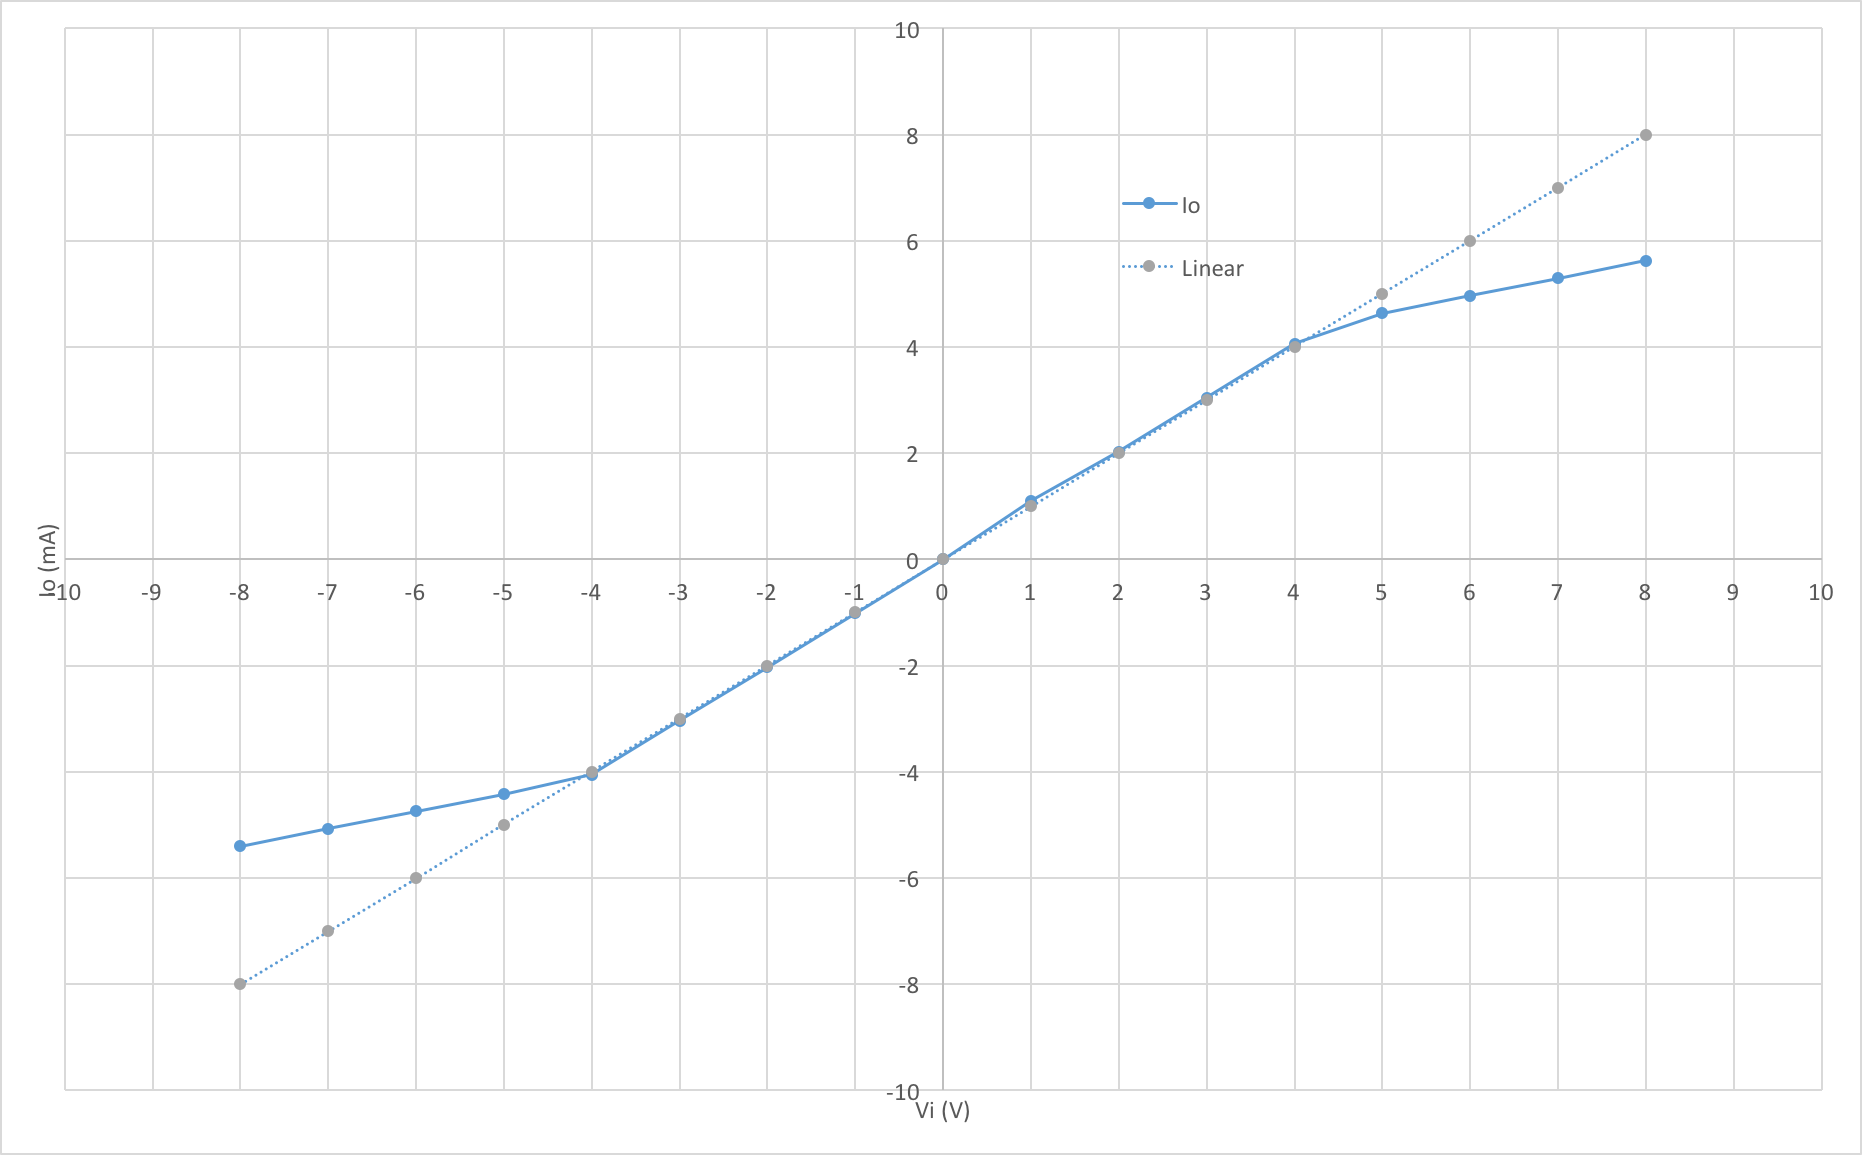
\includegraphics[width=0.95\linewidth]{graphics/vccs-graph}
	\caption{Response characteristic of VCCS with expected linear behavior}
	\label{fig:vccs-graph}
\end{figure}
